\modified{In this section I present the performed study using \sgp{} (\SGP) as a benchmark.}

\subsection{Problem definition}

The \sgp{} (\SGP) consists in scheduling $g\times p$ golfers into $g$ groups of $p$ players every week for $w$ weeks, such that two players play in the same group at most once. An instance of this problem can be represented by the triple $g-p-w$. This problem, and other closely related problems, arise in many practical applications such as encoding, encryption, and covering problems~\cite{Lardeux2014}. Its structure is very attractive, because it is very similar to other problems, like \textit{Kirkman's Schoolgirl Problem} and the \textit{Steiner Triple System}, so efficient modules to solve a broad range of problems can be built.

\modified{The cost function for this} benchmark was implemented making an efficient use of the stored information about the cost of the previews configuration. Using integers to work with bit-flags, a table to store the information about the partners of each player in each week can be filled in $O\left(p^2\cdot g \cdot w\right)$. So, if a configuration has $n = (p\cdot g \cdot w)$ elements, this table can be filled in $O\left(p\cdot n\right)$. This table is filled from scratch only one time in the search process (I explain in the next section why). Then, every cost of a new configuration, is calculated based on this information and the performed changes between the new configuration and the stored one. This relative cost is calculated in $O\left(c\cdot g\right)$, where $c$ is the number of performed changed in the new configuration with respect to the stored one.

\subsection{Experiment design}

Here, I give the \as{} designed for this problem as well as concrete \oms{} composing the different solvers I have tested:

\begin{enumerate}
	\item Generation module:
	\subitem $I$: Generates a random configuration $s$, respecting the structure of the problem, {\it i.e.}, the configuration is a set of $w$ permutations of the vector $[1..n]$. 
	\item Neighborhood modules:
	\subitem $V_{Std}$: Defines the neighborhood $\mathcal{V}\left(s\right)$ swapping players among groups.
	\subitem $V_{AS}$: Defines the neighborhood $\mathcal{V}\left(s\right)$ swapping the most culprit player with other players from the same week. It is based on the {\it Adaptive Search} algorithm.
	\item Selection modules:
	\subitem $S_{First}$: Selects the first configuration $s' \in \mathcal{V}\left(s\right)$ improving the current cost.
	\subitem $S_{Best}$: Selects the best configuration $s' \in \mathcal{V}\left(s\right)$ improving the current cost.
	\subitem $S_{Rand}$: Selects a random configuration $s' \in \mathcal{V}\left(s\right)$.
	\item Acceptance module:
	\subitem $A$: Evaluates an acceptance criteria for $s'$. We have chosen the classical module selecting the configuration with the lowest global cost, {\it i.e.}, the one which is likely the closest to a solution.
\end{enumerate}

A very first experiment was performed to select the best neighborhood function to solve the problem, comparing a basic solver using $V_{Std}$; a new solver using $V_{AS}$; and a combination of $V_{Std}$ and $V_{AS}$ by applying the operators $\circled{$\rho$}$, already introduced in the previous chapter. Algorithms~\ref{as:golfers10-10-3}, \ref{as:golfers_rho} and \ref{as:golfers_union} present the \as{} for each case, respectively.

\begin{algorithm}[H]
\dontprintsemicolon
\SetNoline
\SetKwProg{myproc}{\tet{\bf abstract solver}}{\tet{\bf begin}}{\tet{\bf end}}
\myproc{as\_union \tcp*{{\sc Itr} $\rightarrow$ number of iterations}
	\tet{\bf computation} : $I, V, S, A$\;}{
	\While{$\left(\textbf{\Iter < } K_1\right)$}{%M_1^a \circled{$\rho$} M_1^b
		$I \poslop{\mapsto}$
		\whileinline{$\left(\textbf{\Iter \% } K_2\right)$}{$\left[V \poslop{\mapsto} S \poslop{\mapsto} A\right]$}
	}	
}
\caption{Standard \as{} for \SGP}\label{as:golfers10-10-3}
\end{algorithm}

\begin{algorithm}[H]
\dontprintsemicolon
\SetNoline
\SetKwProg{myproc}{\tet{\bf abstract solver}}{\tet{\bf begin}}{\tet{\bf end}}
\myproc{as\_union \tcp*{{\sc Itr} $\rightarrow$ number of iterations}
	\tet{\bf computation} : $I, V_1, V_2, S, A$\;}{
	\While{$\left(\textbf{\Iter < } K_1\right)$}{%M_1^a \circled{$\rho$} M_1^b
		$I \poslop{\mapsto}$
		\whileinline{$\left(\textbf{\Iter \% } K_2\right)$}{$\left[\left[V_1 \poslop{\rho} V_2\right] \poslop{\mapsto} S \poslop{\mapsto} A\right]$}
	}	
}
\caption{\As{} combining neighborhood functions using operator {\it RHO}}\label{as:golfers_rho}
\end{algorithm}

\begin{algorithm}[H]
\dontprintsemicolon
\SetNoline
\SetKwProg{myproc}{\tet{\bf abstract solver}}{\tet{\bf begin}}{\tet{\bf end}}
\myproc{as\_union \tcp*{{\sc Itr} $\rightarrow$ number of iterations}
	\tet{\bf computation} : $I, V_1, V_2, S, A$\;}{
	\While{$\left(\textbf{\Iter < } K_1\right)$}{%M_1^a \circled{$\rho$} M_1^b
		$I \poslop{\mapsto}$
		\whileinline{$\left(\textbf{\Iter \% } K_2\right)$}{$\left[\left[V_1 \poslop{\cup} V_2\right] \poslop{\mapsto} S \poslop{\mapsto} A\right]$}
	}	
}
\caption{\As{} combining neighborhood functions using operator {\it Union}}\label{as:golfers_union}
\end{algorithm}

Solvers mentioned above were too slow to solve instances of the problem with more than 3 weeks, so another solver implementing the \as{} described in Algorithm~\ref{as:golfers_b001} have been created, using $V_{AS}$ and combining $S_{First}$ and $S_{Rand}$: it tries a number of times to improve the cost, and if it is not possible, it picks a random neighbor for the next iteration. We also compared the $S_{First}$ and $S_{Best}$ selection modules.

\begin{algorithm}[H]
\dontprintsemicolon
\SetNoline
\SetKwProg{myproc}{\tet{\bf abstract solver}}{\tet{\bf begin}}{\tet{\bf end}}
\myproc{as\_eager \tcp*{{\sc Itr} $\rightarrow$ number of iterations}
	\tet{\bf computation} : $I, V, S_1, S_2, A$\;}{
	\While{$\left(\textbf{\Iter < } K_1\right)$}{%M_1^a \circled{$\rho$} M_1^b
		$I \poslop{\mapsto}$
		\whileinline{$\left(\textbf{\Iter \% } K_2\right)$}{$\left[V \poslop{\mapsto} \left[S_1 \poslopcond{\Sci < K_3} S_2\right] \poslop{\mapsto} A\right]$}
	}
}
\caption{\As{} for \SGP{} to scape from local minima}\label{as:golfers_b001}
\end{algorithm}

After that, the best solver to be communicating solvers to compare their performance with the non communicating strategies was chosen. The shared information is the current configuration. Algorithms~\ref{as:golfers_sender}~and~\ref{as:golfers_receiver} show that the communication is performed while applying the acceptance criterion of the new configuration for the next iteration. Here, solvers receive a configuration from an outer solver, and match it with their current configuration. Then solvers select the configuration with the lowest global cost. 
%Using the communication operators, 
We design different communication strategies. Either we execute a full connected solvers set, or a tuned combination of connected and unconnected solvers. Between connected solvers, we applied two different connections operations: connecting each sender solver with one receiver solver ({\it 1~to~1}), or connecting each sender solver with all receiver solvers ({\it 1~to~N}).
%\begin{itemize} %\begin{inparaenum}
%	\item {\it Full communication strategy}: all solvers are connected (either {\it 1 to 1}, or {\it 1 to N})
%	\item \textit{Hybrid communication strategy}: A given percentage of solvers are connected and the others are non communicating solvers.
%\end{itemize} %\end{inparaenum}

\begin{algorithm}
\dontprintsemicolon
\SetNoline
\SetKwProg{myproc}{\tet{\bf abstract solver}}{\tet{\bf begin}}{\tet{\bf end}}
\myproc{as\_eager\_sender \tcp*{{\sc Itr} $\rightarrow$ number of iterations}
	\tet{\bf computation} : $I, V, S_1, S_2, A$\tcp*{{\sc Sci} $\rightarrow$ number of iterations with the same cost}}{%	
	\While{$\left(\textbf{\Iter < } K_1\right)$}{%M_1^a \circled{$\rho$} M_1^b
		$I \poslop{\mapsto}$
		\whileinline{$\left(\textbf{\Iter \% } K_2\right)$}{$\left[V \poslop{\mapsto} \left[S_1 \poslopcond{\Sci < K_3} S_2\right] \poslop{\mapsto} \llparenthesis A \rrparenthesis^o\right]$}
	}
}
\caption{Communicating \as{} for \SGP{} (sender)}\label{as:golfers_sender}
\end{algorithm}

\begin{algorithm}
\dontprintsemicolon
\SetNoline
\SetKwProg{myproc}{\tet{\bf abstract solver}}{\tet{\bf begin}}{\tet{\bf end}}
\myproc{as\_eager\_receiver \tcp*{{\sc Itr} $\rightarrow$ number of iterations}
	\tet{\bf computation} : $I, V, S_1, S_2, A$\tcp*{{\sc Sci} $\rightarrow$ number of iterations with the same cost}
	\tet{\bf communication} : $C.M.$\;}{%	
	\While{$\left(\textbf{\Iter < } K_1\right)$}{%M_1^a \circled{$\rho$} M_1^b
		$I \poslop{\mapsto}$\\
		\While{$\left(\textbf{\Iter \% } K_2\right)$}{
			$ V \poslop{\mapsto} \left[S_1 \poslopcond{\Sci < K_3} S_2\right] \poslop{\mapsto} \left[A \poslop{m} C.M.\right]$
		}
	}
}
\caption{Communicating \as{} for \SGP{} (receiver)}\label{as:golfers_receiver}
\end{algorithm}

%Obviously, the communication frequency have to be controlled, because it can slow down the search process. %\posl{} provides the conditional operator $\circled{?}$ that executes its first or second parameter, depending its given boolean criterion is true or not.

\modified{In all Algorithms} ins this section, three parameter can be found:\begin{inparaenum}[1.] \item $K_1$: the maximum number of {\it restarts}, \item $K_2$: the maximum number of iterations in each \textit{restart}, and $K_3$: the maximum number of iterations with the same current cost. \item \end{inparaenum}

\modified{After the selection of the proper modules to study different communication strategies, I proceeded to tune these parameter. Only a few runs were necessaries to conclude that the mechanism of using the \om{} $S_{rand}$ to scape from local minima was enough. For that reason, since the solver never perform restarts, the parameter $K_1$ was irrelevant. So the reader can assume $K_1 = 1$ for every experiment.}

\modified{With the certainty that solvers do not performs restarts during the search process, I select the same value for $K_2 = 5000$ in order to be able to use the same \as{} for all instances.}

\modified{Finally, in the tuning process of $K_3$, I notice only slightly differences between using the values $5$, $10$, and $15$. So I decided to use $K_3 = 5$.}

%--------------------------------------------------------------------------
%----- R E S U L T S
%--------------------------------------------------------------------------
\subsection{Analysis of results}

Table~\ref{tab:golfers_seq} showed results of launching \soset s to solve each instance of the problem sequentially. Not surprisingly, the means of sequential runtimes and iterations (Table~\ref{tab:golfers_seq}) are bigger than those means of parallel runs, with or without communication (all other tables). 
%This confirms the intuition that parallel approach increases the probability of finding the solution within a more reasonable time (some tens of seconds), than with the sequential scheme \cite{Alon2011}. 
%The column labeled \textbf{\% success} in Table~\ref{tab:golfers_seq} indicates the percentage of solvers finding a solution before reaching a time--out (5 minutes). 
%presented in Table~\ref{tab:golfersB001}, column \textit{O.M. First Improvement} (without communication), and results with communication (Tables~\ref{tab:golfersB001comm100}, \ref{tab:golfersB001comm50} and \ref{tab:golfersB001comm25}). 

\begin{table}[h]
\centering
\renewcommand{\arraystretch}{1}
\begin{tabular}{p{1.5cm}|R{1.5cm}R{1.5cm}R{1.5cm}R{1.5cm}R{2.5cm}}
\hline
{\bf Instance} & T & T(sd) & It. & It.(sd) & \% success\\
\hline
%\hline
5--3--7 & 8.31 & 7.64 & 17,347 & 15,673 & 100.00\\
8--4--7 & 16.92 & 15.15 & 7,829 & 7,019 & 100.00\\
9--4--8 & 79.60 & 64.07 & 20,779 & 16,537 & 94.28\\
11--7--5 & 3.37 & 2.16 & 664 & 380 & 100.00\\
\hline
\end{tabular}
\caption{\sg: a single sequential solver}
\label{tab:golfers_seq}
\end{table}

In a first stage of the experiments I use the operator-based language provided by \posl{} to build and test many different non communicating strategies. The goal is to select the best concrete modules to run tests performing communication. In particular, I have tested two kind of computation modules: the one computing the neighborhood of a given configuration and the one choosing the current configuration for the next solver iteration.

I focused on choosing the right neighborhood function. In the case of the \sgp, this experiment was launched using a basic abstract solver showed in Algorithm~\ref{as:golfers10-10-3}.
Solvers implemented from this abstract solver was too slow to solve instances beyond three weeks: they were very often trapped into local minima. This is the reason why we perform this first experiment with the instance 10--10--3 whereas next experiments scale above 3 weeks. This was not a problem though, since the goal of this first experiment was only to find the right concrete neighborhood module.

\begin{table}
\centering 
\renewcommand{\arraystretch}{1}
\begin{tabular}{p{4cm}|R{1.3cm}R{1.3cm}R{1.3cm}R{1.3cm}}
\hline
{\bf Abstract solvers} & T & T(sd) & It. & It.(sd) \\
\hline
%\hline
Adaptive Search (AS) & \good{\bf 1.06} & 0.79 & 352 & 268 \\		
Std $\circled{$\rho$}$ AS & 41.53 & 26.00 & 147 & 72\\
Std $\circled{$\cup$}$ AS & 59.65 & 55.01 & 198 & 110\\
Standard (Std) & 87.90 & 41.96 & 146 & 58 \\
\hline
\end{tabular}
\caption{\sg: Instance 10--10--3 in parallel}
\label{tab:golfers10-10-3}
\end{table}

Results in Table~\ref{tab:golfers10-10-3} are not surprising. The neighborhood module $V_{AS}$ is based on the {\it Adaptive Search} algorithm, which has shown very good results \cite{Diaz}. %It selects the variable (player) contributing the most to the cost and permutes its value with the others variables (players) for all groups, every week.
It selects the most culprit variable (i.e., a player), that is, the variable to most responsible for constraints violation. Then, it permutes this variable value with the value of each other variable, in all groups and all weeks. Each permutation gives a neighbor of the current configuration. $V_{Std}$ uses no additional information, so it performs every possible swap between two players in different groups, every week. It means that this neighborhood is $g\times p$ times bigger than the previous one, with $g$ the number of groups and $p$ the number of players per group. 
\modified{It allows for more organized search because the set of neighbors is pseudo-deterministic, i.e., the construction criteria is always the same but the order of the configuration is random. On the other hand, {\it Adaptive Search} neighborhood function takes random decisions more frequently, and the order of the configurations is random as well.}
We also tested abstract solvers with different combinations of these modules, using the $\circled{$\rho$}$ and the $\circled{$\cup$}$ operators. The $\circled{$\rho$}$ operator executes its first or second parameter depending on a given probability $\rho$, and the $\circled{$\cup$}$ operator returns the union of its parameters output. All these combinations spent more time searching the best configuration among the neighborhood, although with a lower number of iterations than $V_{AS}$. The $V_{AS}$ neighborhood function being clearly faster, we have chosen it for our experiments, even if it shown a more spread standard deviation: 0.75 for AS versus 0.62 for Std, considering the ratio $\tfrac{T(sd)}{T}$.

\begin{table}
\captionsetup{belowskip=6pt,aboveskip=6pt}
\centering 
\renewcommand{\arraystretch}{1}
\begin{tabular}{p{2cm}|R{1cm}R{1cm}R{1cm}R{1.2cm}|R{1cm}R{1cm}R{1cm}R{1.2cm}}
	\hline %\noalign{\smallskip}	
	\multirow{2}{*}{\footnotesize{\centering {\bf Instance}}} & 
	\multicolumn{4}{c|}{O.M. Best Improvement} & 
	\multicolumn{4}{c}{O.M. First Improvement}\\
	\cline{2-9} %\cline{3-8}
	& T & T(sd) & It. & It.(sd) & T & T(sd) & It. & It.(sd) \\
	\hline
	%\hline
	5--3--7 & 4.99 & 4.43 & 4,421 & 3,938 & \good{\bf 1.32} & 0.68 & 1322 & 676\\
	8--4--7 & 5.10 & 1.77 & 954 & 334 & \good{\bf 1.82} & 0.84 & 445 & 191\\	
	9--4--8 & 12.37 & 5.40 & 1,342 & 591 & \good{\bf 6.43} & 4.60 & 873 & 591 \\
	11--7--5 & 5.19 & 1.67 & 351 & 114 & \good{\bf 2.22} & 0.69 & 273 & 58\\
	\hline
\end{tabular}
\caption{\sg: comparing selection functions}
\label{tab:golfersB001}
\end{table}

With the selected neighborhood function, I focused on choosing the best {\it selection} function. I compared two different concrete modules used within the abstract solver in Algorithm~\ref{as:golfers_b001}, which combines selection modules ($S_{First}$ or $S_{Best}$) with $S_{Rand}$, to avoid being trapped into local minima: it tries to improve the cost in a limited number of iterations. If it is not possible, it selects a random neighbor for the next iteration. The first module was $S_{Best}$ that selects the best configuration inside the neighborhood. It not only spent more time searching a better configuration, but also is more sensitive to become trapped into local minima. The second module was $S_{First}$ which selects the first configuration inside the neighborhood improving the current cost. Using this module, solvers favor exploration over intensification and of course spend clearly less time computing the neighborhood. Table~\ref{tab:golfersB001} presents results of this experiment, showing that an exploration-oriented strategy is better for the \SGP. If we compare results of Tables~\ref{tab:golfers_seq} and \ref{tab:golfersB001} with respect to the standard deviation, we can some gains in robustness with parallelism. The spread in the running times and iterations for the instance 9--4--8 (the hardest one) is 10\% lower (0.80 sequentially versus 0.71 in parallel), and for the others, it is around 40\% lower (0.91, 0.89 and 0.64 sequentially versus 0.51, 0.45 and 0.31 in parallel, for 5--3--7, 8--4--7 and 11--7--5 respectively, with the same ratio $\tfrac{T(sd)}{T}$).

\begin{table}
	\captionsetup{belowskip=6pt,aboveskip=6pt}
	\centering 
	\renewcommand{\arraystretch}{1}
		\begin{tabular}{p{2cm}|R{1cm}R{1cm}R{1cm}R{1.2cm}|R{1cm}R{1cm}R{1cm}R{1.2cm}}
			\hline 	
			\multirow{2}{*}{\centering {\bf Instance}} & \multicolumn{4}{c}{Communication 1 to 1} & \multicolumn{4}{c}{Communication 1 to N}\\
			\cline{2-9}
			& T & T(sd) & It. & It.(sd) & T & T(sd) & It. & It.(sd) \\
			\hline
			%\hline
			5--3--7 & 1.19 & 0.64 & 1,156 & 608 & 1.11 & 0.49 & 1,067 & 484\\
			8--4--7 & \good{1.30} & 0.72 & \good{317} & 161 & 1.46 & 0.57 & 347 & 128\\
			9--4--8 & 4.38 & 2.72 & \good{597} & 347 & 5.51 & 3.06 & 736 & 389\\
			11--7--5 & 1.76 & 0.41 & 214 & 44 & \good{1.62} & 0.34 & \good{202} & 30\\
			\hline
		\end{tabular}
	\caption{\sg: test with 100\% of communication}
	\label{tab:golfersB001comm100}
\end{table}

\begin{table}
	\captionsetup{belowskip=6pt,aboveskip=6pt}
	\centering 
	\renewcommand{\arraystretch}{1}
		\begin{tabular}{p{2cm}|R{1cm}R{1cm}R{1cm}R{1.2cm}|R{1cm}R{1cm}R{1cm}R{1.2cm}}
			\hline 	
			\multirow{2}{*}{\centering {\bf Instance}} & \multicolumn{4}{c}{Communication 1 to 1} & \multicolumn{4}{c}{Communication 1 to N}\\
			\cline{2-9}
			& T & T(sd) & It. & It.(sd) & T & T(sd) & It. & It.(sd) \\
			\hline
			%\hline
			5--3--7 & 1.04 & 0.45 & 1,019 & 456 & 1.04 & 0.53 & 1,031 & 530\\
			8--4--7 & 1.40 & 0.57 & 337 & 122 & 1.43 & 0.76 & 353 & 167\\
			9--4--8 & 4.64 & 2.17 & 637 & 279 & 5.75 & 3.06 & 776 & 389 \\
			11--7--5 & 1.81 & 0.40 & 220 & 33 & 1.82 & 0.39 & 222 & 39\\
			\hline
		\end{tabular}
	\caption{\sg: test with 50 \% of communication}
	\label{tab:golfersB001comm50}
\end{table}

\begin{table}
	\captionsetup{belowskip=6pt,aboveskip=6pt}
	\centering 
	\renewcommand{\arraystretch}{1}
		\begin{tabular}{p{2cm}|R{1cm}R{1cm}R{1cm}R{1.2cm}|R{1cm}R{1cm}R{1cm}R{1.2cm}}
			\hline 	
			\multirow{2}{*}{\centering {\bf Instance}} & \multicolumn{4}{c}{Communication 1 to 1} & \multicolumn{4}{c}{Communication 1 to N}\\
			\cline{2-9}
			& T & T(sd) & It. & It.(sd) & T & T(sd) & It. & It.(sd) \\
			\hline
			%\hline
			5--3--7 & \good{0.90} & 0.51 & \good{881} & 492 & 1.19 & 0.67 & 1,170 & 655\\
			8--4--7 & 1.39 & 0.43 & 341 & 94 & 1.46 & 0.43 & 352 & 96\\
			9--4--8 & \good{4.33} & 1.92 & 599 & 248 & 4.53 & 2.01 & 625 & 251\\
			11--7--5 & 1.99 & 0.54 & 242 & 51 & 1.63 & 0.35 & 224 & 28 \\
			\hline
		\end{tabular}
	\caption{\sg: test with 25\% of communication}
	\label{tab:golfersB001comm25}
\end{table}

\modified{Then we ran experiments to study \posl's behavior solving target problems in communicating scenarios. Some compositions of solvers set were taken into account:}
\begin{inparaenum}[i.]
	\item the structure of the communication (with/without communication or a mix), and
	\item \modified{the used communication operator}.
\end{inparaenum}

Each time a \posl{} meta-solver is launched, many independent search solvers are executed. We call "good" configuration a configuration with the lowest cost within the current configuration neighborhood and with a cost strictly lesser than the current one. Once a good configuration is found in a sender solver, it is transmitted to the receiver one. At this moment, if the information is accepted, there are some solvers searching in the same subset of the search space, and the search process becomes more exploitation--oriented. This can be problematic if this process makes solvers converging too often towards local minima. In that case, we waste more than one solver trapped into a local minima: we waste all solvers that have been attracted to this part of the search space because of communications. I avoid this phenomenon through a simple (but effective) play: if a solver is not able to find a better configuration inside the neighborhood (executing $S_{First}$), it selects a random one at the next iteration (executing $S_{Rand}$). This strategy, using communication between solvers, produces some gain in terms of runtime (Table~\ref{tab:golfersB001} with respect to Tables~\ref{tab:golfersB001comm100}, \ref{tab:golfersB001comm50} and \ref{tab:golfersB001comm25}. The percentage of the receiver solvers that were able to find the solution before the others did, was significant (see Appendix~\ref{app:sgp}).
That shows that the communication played an important role during the search, despite inter--process communication's overheads (reception, information interpretation, making decisions, etc). 
\modified{Having many solvers searching in different places of the search space, the probability that one of them reaches a promising place is higher. Then, when a solver finds a good configuration, it can be communicated, and receiving the help of one or more solvers in order to find the solution.}
For this problem we have reduced the spread in the running times and iterations of the results for the two last instances (9--4--8 and 11--7--5) applying the communication strategy (0.71 without communication versus 0.44 with communication, for 9--4--8, and 0.31 without communication versus 0.20 with communication for 11--7--5).

\modified{Other two} strategies were analyzed in the resolution of this problem, with no success, both based on the sub-division of the work by weeks, i.e., solvers trying to improve a configuration only working with one or some weeks. To this end two strategies were designed:

\begin{enumerate}[label=\Alph*]
\item \textbf{Circular strategy:} $K$ solvers try to improve a configuration during a during a number of iteration, only working on one week. When no improvement is obtained, the current configuration is communicated to the next solver (circularly), which tries to do the same working on the next week (see Figure~\ref{subfig:golfers_bad_ring}).
\subitem This strategy does not show better results than previews strategies. The reason is because, although the communication in \posl{} is asynchronous, most of the times solvers were trapped waiting for a configuration coming from its neighbor solver.

\item \textbf{Dichotomy strategy:} Solvers are divided by levels. Solvers in level 1, only work on one week, solvers on level 2, only work on 2 consecutive weeks, and so on, until the solver that works on all (except the first one) weeks. Solvers in level 1 improve a configuration during some number of iteration, then this configuration is sent to the corresponding solver. A solver in level 2 do the same, but working on weeks $k$ to $k+1$. It means that it receives configurations from the solver working on week $k$ and from the solver working on week $k+1$, and sends its configuration to the corresponding solver working on weeks $k$ to $k+3$; and so on. The solver in the last level works on all (except the first one) weeks and receive configuration from the solver working on weeks $2$ to $w/2$ and from the solver working on weeks $w/2+1$ to $w$ (see Figure\ref{subfig:golfers_bad_dic}). We tested this strategy with all possible levels. 
\subitem The goal of this strategy was testing if focused searches rapidly communicated can help at the beginning of the search. However, The failure of this strategy is in the fact that most of the time the sent information arrives to late to the receiver solver.
\end{enumerate}

\begin{figure}[h]
	\centering
	\subfloat[][]{
		\label{subfig:golfers_bad_ring}
		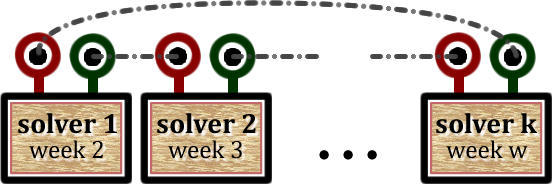
\includegraphics[width=0.45\linewidth]{golfers_ring.png}
	} %\hspace{0.1\linewidth}
	\subfloat[][]{%
		\label{subfig:golfers_bad_dic}
		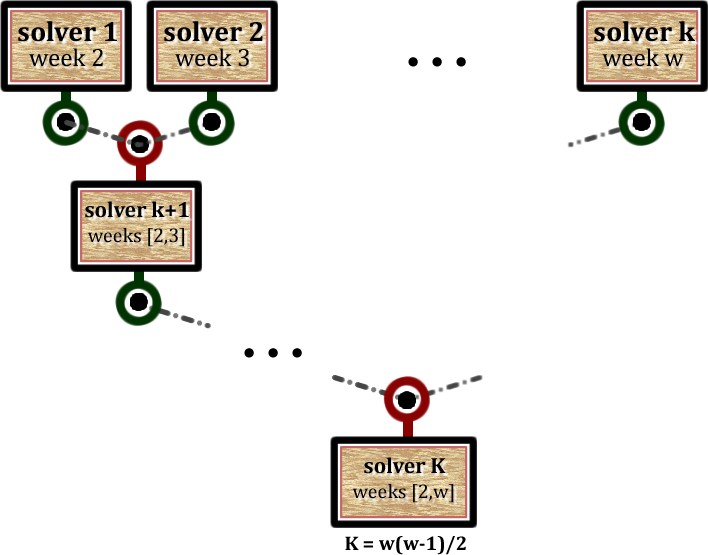
\includegraphics[width=0.45\linewidth]{golfers_dic.png}
	}
	\caption[]{Unsuccessful communication strategies to solve \SGP}
	\label{fig:golfers_bad}
\end{figure}